\section{Abstractions for NDA}
\label{sec:abstractions}

\begin{quote}
{\em Synthesis implies a bridge between two layers of abstraction} -- A. Sangiovanni-Vincentelli~\cite{alberto}
\vspace{-2mm}
\end{quote}

\begin{figure}[t]
\centerline{
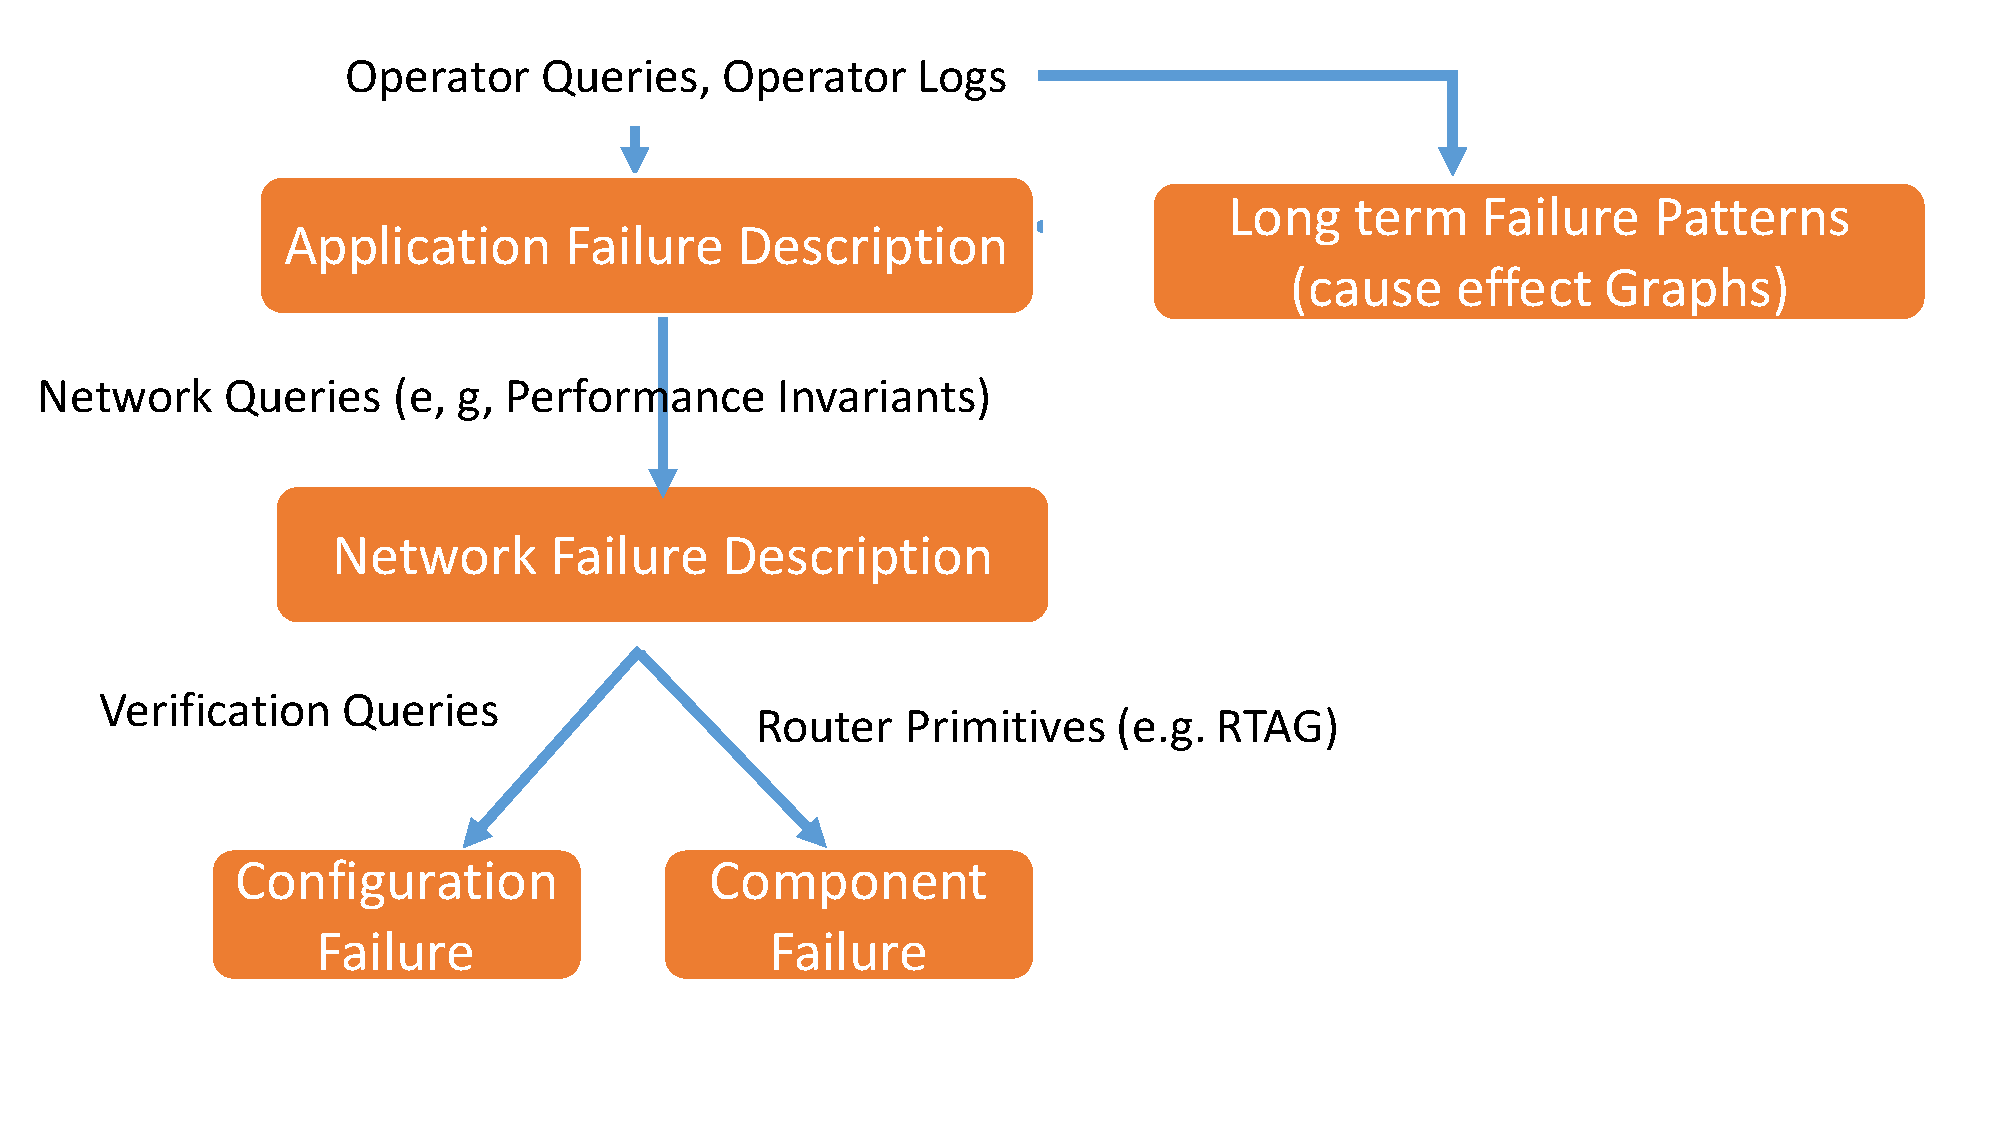
\epsfig{file=NDA-abstractions-new.pdf, height=4in}
}
\caption{\label{fig:abstractions} The layers of abstraction in NDA.}
\vspace{-5mm}
\end{figure}

Abstractions were key to the success of EDA~\cite{malik}. For example, EDA includes abstractions for high-level behavioral models, blocks, logic gates, and finally wires.  Such abstractions then support both {\em bottom-up verification}, from a lower-level abstraction to a higher-level one, and {\em top-down synthesis}, from a higher-level abstraction to a lower-level one.  

Analogously, our technical work will be driven by an interconnected set of abstractions for both network design and network debugging.
Networks already have
abstractions for packet delivery (TCP and IP~\cite{kurose}) and for
packet forwarding (SDN-inspired flow
rules~\cite{Ethane,4DControlPlane,shenker-abstractions}) but lack general abstractions for network design/configuration and for systems-level debugging.

\paragraph*{Abstractions for Network Design}
%
The two abstraction levels for network design are related to {\em topology} and {\em configuration}. An abstraction for topology would allow for specification of high-level topology policies and requirements, including resiliency requirements and traffic forecasts.  Given such an abstraction, we envision a tool that can automatically produce a corresponding physical network. Many cloud providers including Google~\cite{condor} and Microsoft already have these kinds of tools but they are very specific to data-center networks and the particular needs of the organization.  Our goal is to develop expressive abstractions for topology policy/requirements for a broad range of networks -- from data centers to CDNs to rural networks -- along with tools to produce physical networks that meet these specifications.

% Imagine an open source tool that can design a physical network whether
% for a rural network that uses VoIP (1000 users in 12 villages, using wireless links and FPGA based routers) or a larger data center network for Google (10, 000 users for Google Applications using high end Cisco routers) or a CDN. The Condor system at
% Google~\cite{condor} recently proposed a delarative Topology
% Description Language (TDL) to specify abstract topology connectivity
% and uses a constraint solver to generate topologies but it only automates
% some limited aspects of topology design.

The next layer of abstraction is a description of the network's {\em routing policy}.  We will design expressive abstractions that support both global requirements that must hold of the network as a whole as well as local requirements that must hold of an individual router.  These abstractions will then form the basis for new tools for verifying and synthesizing network configurations.  Rather than directly verifying or synthesizing vendor-specific configuration files, we will leverage existing vendor-independent configuration abstractions such as 
Open Config~\cite{openconfig} and the intermediate representation in the open-source Batfish~\cite{batfish} tool that PI Millstein has developed.  

\paragraph{Abstractions for Network Debugging}  Even if a network is synthesized to satisfy a given policy, there will always be properties that cannot be verified during synthesis, and the needs of the network evolve over time due to new requirements and constraints.  Thus to complement our work on network design we will pursue an interconnected set of abstractions for system-level debugging.
We have identified an initial set of abstraction layers that will frame our proposed debugging research
(Figure~\ref{fig:abstractions}): {\em application failure description}, {\em network failure description},  
{\em configuration failure description}, and {\em component failure description}.  The idea is to map 
from the highest layer (application failures) to lower level culprits (configurations, components) by a set
of interconnected tools.

First, note that higher level operator concerns and problems are often expressed in operator logs.  While
we will also design a language to express operator concerns (e.g., SLA violations), we feel it is also
important to map from operator logs to application problems.
Next, we need to connect the abstract, high-level application failure language to the
low-level, structured query languages that express network failures (e.g., Marple~\cite{marple} or 
our proposal for  performance invariants).  Finally, we isolate the issue when possible to 
either a configuration failure (that can be detected by configuration verification tools (e.g., Minesweeper\cite{minesweeper} or enhacements we describe later) or router primitives (e.g., packet mirroring as in
Everflow or RTAG as we describe later).

 On a longer time scale, the
network architect also needs to extract, from logs of network faults
captured (often annotated by a network operator), a higher-level
{\em failure model}, which can be used to target efforts to improve
reliability. 

\paragraph*{Our Proposed Work} While there exist point solutions at some of
these layers for certain tasks, these abstractions are neither {\em
  complete} or {\em interconnected}. We will produce a complete and
interconnected set of abstractions for network design and debugging.
Section~\ref{sec:approaches} describes our proposed work
in detail and sets it in the context of related work.
%
% In the following paragraphs, we discuss our
% research in synthesis and verification, achieved through pairwise
% inter-disciplinary collaborations.
%
Our focus is on designing specialized networks within a single
Autonomous System (AS), where the architect and operator can control the 
entire network.  Of course, individual networks are interconnected to form the Internet.  Network Design Automation ``in the large,'' across multiple ASes, is out of scope for our project.





 
